\section{An Extended OCL for Temporal and Event Specifications}

%%%%% TOCL
\subsection{Adopted TOCL Temporal Operators}

\hspace{1cm} TOCL (Temporal OCL), introduced by Ziemann and Gogolla \cite{TOCL}, 
extends OCL with temporal operators for specifying properties that must hold across 
multiple system states. It incorporates elements of linear temporal logic while 
maintaining OCL's familiar syntax, enabling developers to express temporal constraints 
directly within their models. TOCL extends standard OCL with a comprehensive set of 
temporal operators categorized into future operators (next, always, sometime, until, 
before) and past operators (previous, alwaysPast, sometimePast, since), each with 
well-defined semantics for reasoning about system behavior over time. These operators 
follow the principles of linear temporal logic but are adapted to work within OCL's 
object-oriented context, preserving OCL's typing system and navigation capabilities. 
By integrating temporal reasoning directly into OCL, TOCL provides a unified formalism 
that addresses the fundamental limitations of standard OCL when specifying dynamic 
system aspects, particularly those involving sequences of states or temporal 
relationships between conditions.

In our work, we adopt the following temporal operators from TOCL:

\paragraph{Future Operators:} 
\begin{itemize} 
    \item \textbf{next $e$:} True if the expression $e$ holds in the next state. 
    \item \textbf{always $e$:} True if $e$ holds in the current state and all subsequent states. 
    \item \textbf{sometime $e$:} True if $e$ holds in the current state or at least one future state. 
    \item \textbf{always $e_1$ until $e_2$:} True if $e_1$ remains true until $e_2$ becomes true, or if $e_1$ remains true indefinitely if $e_2$ never becomes true. 
    \item \textbf{sometime $e_1$ before $e_2$:} True if $e_1$ becomes true at some point before $e_2$ does, or if $e_1$ becomes true and $e_2$ never does. 
\end{itemize}

\paragraph{Past Operators:} \begin{itemize} 
    \item \textbf{previous $e$:} True if $e$ was true in the previous state (or if there is no previous state, i.e., at the initial state). 
    \item \textbf{alwaysPast $e$:} True if $e$ was true in all past states. 
    \item \textbf{sometimePast $e$:} True if $e$ was true in at least one past state. 
    \item \textbf{always $e_1$ since $e_2$:} True if $e_1$ has been true since the last time $e_2$ was true. 
    \item \textbf{sometime $e_1$ since $e_2$:} True if $e_1$ has been true at some point since the last time $e_2$ was true. 
\end{itemize}
For the formal semantics of these operators, we refer to the original work by Ziemann and Gogolla \cite{TOCL}.

To illustrate the capabilities of these operators, we will specify the temporal 
properties of the Software System introduced in Chapter 1 (Figure \ref{fig:temporal_properties}).
using TOCL.
\begin{lstlisting}[
    style=toclstyle, 
    caption={TOCL Specification for Safety 1 and 2 property.}, 
    label={lst:tocl_safety12}
]
context System 
/*
An application loading must precede its run.
*/
inv safety1: 
    self.runningApps->notEmpty() implies 
    self.runningApps->forAll(app | 
        sometimePast self.loadedApps->includes(app)
    )
/*
There must be an install operation between an application's loading and its running.
*/
inv safety2: 
    self.loadedApps->notEmpty() implies 
    self.loadedApps->forAll(app | 
        sometime self.installedApps->includes(app) 
        before self.runningApps->includes(app)
    )
\end{lstlisting}
As shown in Listing \ref{lst:tocl_safety12}, TOCL allows us to elegantly express 
properties that span multiple system states. Safety 1 uses the \texttt{sometimePast} 
operator to verify that any application in the \texttt{runningApps} collection must 
have previously been in the \texttt{loadedApps} collection, capturing the temporal 
ordering requirement. Safety 2 utilizes the \texttt{before} operator to specify that 
an application must be in the \texttt{installedApps} collection before it appears 
in the \texttt{runningApps} collection. These specifications are impossible to 
formulate in standard OCL, which has no operators for referring to past or future 
states beyond a single transition.

However, TOCL still has important limitations when it comes to specifying event-based 
properties. For Safety 3 ("Each application can be loaded at most one time"), TOCL 
lacks the ability to detect and count specific occurrences of events like operation 
calls. While TOCL can express that certain conditions hold across states, it doesn't 
offer a direct way to identify the specific moments when operations are called or 
when state changes happen. This limitation becomes particularly problematic when we 
need to express constraints on the number of times an event occurs or when we need 
to detect specific state changes.

%%%%% Event
\subsection{Event Constructs in OCL}

\hspace{1cm} To address TOCL's limitations in expressing event-based properties, we 
propose TOCL+, an extension that introduces explicit event specification capabilities. 
We adopt the concept of events from \cite{TemporalAndEventOCL}, which defines events 
as predicates identifying specific instants in time. As discussed in Section 
\ref{sec:ocl}, object-oriented systems typically recognize multiple event types: 
operation events (call/start/end), time-triggered events, and state change events. 
Our extension focuses specifically on operation and state change events, as they 
capture the fundamental interactions in object-oriented systems.

Following the synchronous paradigm for its well-defined formal semantics, TOCL+ 
merges operation events (call/start/end) into a single construct named 
\texttt{isCalled}. This construct represents the atomic transition from a pre-state 
to a post-state without intermediate states, providing a clean abstraction for 
verification. This atomicity assumption simplifies reasoning about system behavior 
while still capturing essential reactive properties.

TOCL+ introduces two primary event constructs. The first construct, \textbf{isCalled}, 
is a generic event construct that unifies operation events. It detects when an 
operation is invoked on an object, representing the atomic transition from a 
pre-state to a post-state. It has one required parameter, \texttt{op}, which is the 
operation being called with its parameters.

The second construct, \textbf{becomesTrue}, represents a state change event 
parameterized by an OCL boolean expression P. It designates a step in which P becomes 
true (i.e., P was evaluated to false in the previous state and is true in the current 
state).

Both event constructs are illustrated in Figure \ref{fig:event_constructs}.

% Event figures
\begin{figure}
    \centering
    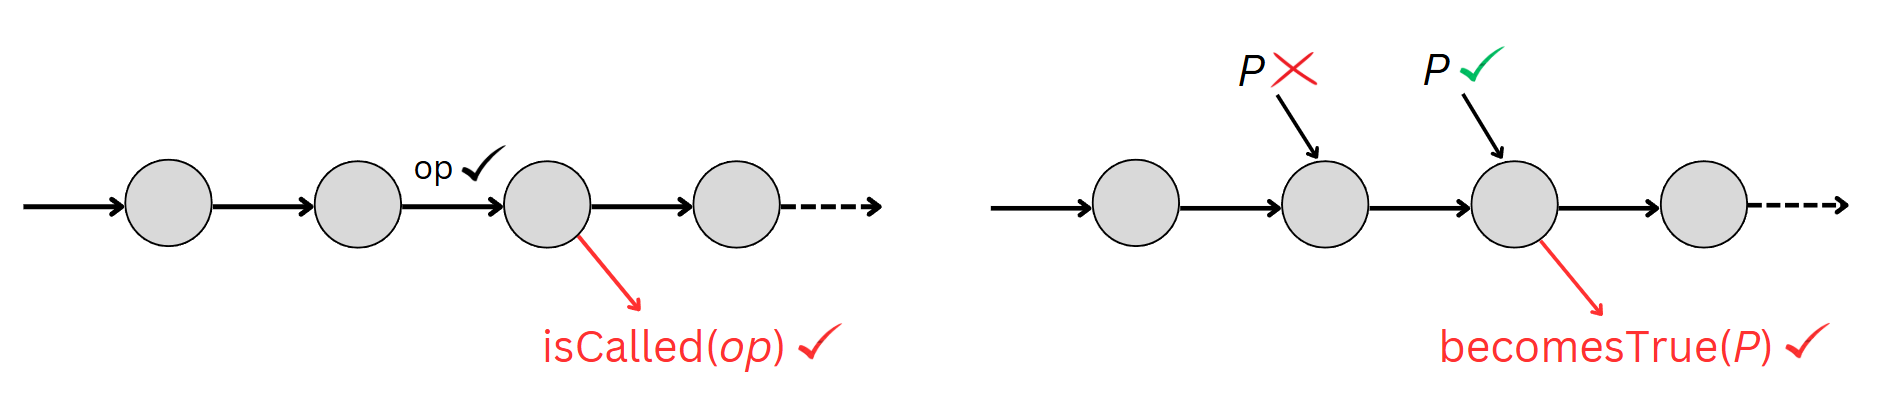
\includegraphics[width=1\textwidth]{figures/c2/events_visual.png}
    \caption{Event constructs in OCL.}
    \label{fig:event_constructs}
\end{figure}


\subsubsection{Formal Definition}

Formally, we define events in terms of operations and state transitions. Let O be the set of all operations and E be the set of all OCL boolean expressions in a model. An event is either:

\begin{itemize}
    \item isCalled(op) - representing a call to operation op, optionally with precondition pre and postcondition post
    \item becomesTrue(P) - representing any operation call that transitions the system from a state where ¬P holds to a state where P holds
\end{itemize}

This formal definition enables precise reasoning about when events occur during system execution and forms the foundation for our verification approach.



%%% Sample
% Events are predicates to specify sets of instants within the time line. In Section 1.4.2, we discussed the different types of
% events in the object-oriented approach. There are operation (call/start/end) events, time-triggered events and state change
% events. We have seen that when integrating the clock into the system, time-triggered events are particular state change
% events. Hence, we only need to extend OCL with the necessary construct for both operation and state change events.
% We aim to connect our OCL temporal extension to formal methods such as model-checking and test scenario generation.
% Formal methods are mainly based on the synchronous paradigm that has well-founded mathematical semantics and that
% allows formal verification of the programs and automatic code generation. The essence of the synchronous paradigm is the
% atomicity of reactions (operation calls) where all the occurring events during such a reaction are considered simultaneous.
% In our work, we adopt the synchronous paradigm, and we merge the operation (call/start/end) events into one call event,
% named isCalled, that leads the system from a pre-state to a post-state without considering neither observing intermediate
% change states.
% isCalled: is a generic event construct that unifies both operation events and state change events.
% becomesTrue: is a state change event that is parameterized by an OCL boolean expression P, and designates a step in
%  which P becomes true, i.e. P was evaluated to false in the previous state. In the object-oriented paradigm, a state change
%  is necessarily a consequence of some operation call, therefore the becomesTrue construct is a syntactic sugar and stands for
%  any operation call switching P to true.
% Formal semantics
% A test case is a scenario in which a set of operations is executed in sequence with observations either before or after each
%  operation execution. Since we are interested in test cases generation (see Section 10), we adopt a scenario-based semantics
%  over the synchronous paradigm to formalize our temporal extension. The essence of that paradigm is the atomicity of
%  reactions (operation calls) where all the events occurring during such a reaction are considered as simultaneous. A reaction
%  is one atomic call event, that leads the system directly from a pre-state to a post-state without going through intermediate
%  states.
% We define the set of all atomic events of a given object model as follows:
% Definition6.1 (Alphabetofatomicevents). Let O be the set of all operations and E be the set of all OCL boolean expressions of
%  an object model M.ThealphabetΣM ofatomicevents (abbreviated as Σ in the following) is defined by the set O×E×E.
%  An atomic event e ∈Σ takes the form: e =(op). It stands for a call of the operation op in a context where pre
%  stands for the precondition satisfied in the pre-state and post stands for the postcondition satisfied in the post-state.
%  We now give the formal meaning of the notion of events introduced in our OCL temporal extension.
%  Definition 6.2 (Events). Let Σ be the alphabet of atomic events, O be the set of all operations and E the set of all OCL
%  boolean expressions. An event is either an isCalled(op,pre,post) or a becomesTrue(P) with:
%  isCalled(op,pre,post) = op,pre,post ∈ Σ pre⇒pre, post⇒post and
%  becomesTrue(P) = (op,pre,post) ∈ Σ op∈O, pre⇒¬P, post⇒ P
%  Definition 6.2 calls for the following comments:– An event does not represent a single atomic event, but a specific subset of atomic events. It is intuitively the set of all
%  atomic events in which the operation op is invoked, in a pre-state which implies the expression pre and leading to a
%  post-state which implies the expression post. The set of all events is then defined6 as the set 2Σ;
